
\documentclass{standalone}
\usepackage{xcolor}
\usepackage{pgfplots}
\pgfplotsset{compat=1.18}

\begin{document}

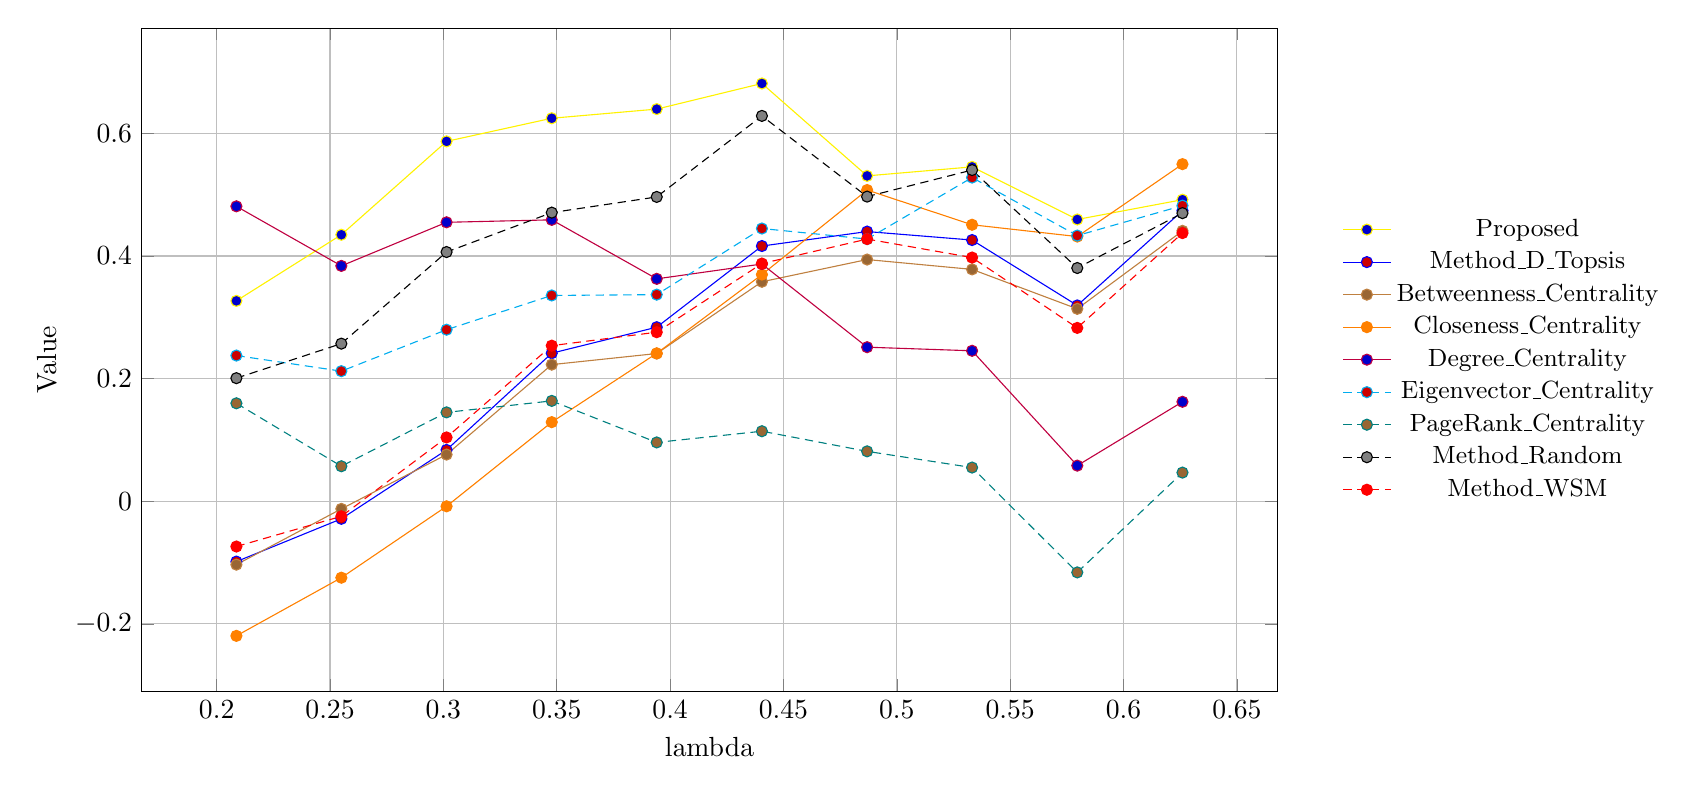
\begin{tikzpicture}
\begin{axis}[
    width=16cm,
    height=10cm,
    xlabel={lambda},
    ylabel={Value},
    grid=major,
    legend style={
        at={(1.05,0.5)},
        anchor=west,
        font=\small,
        draw=none,
        cells={align=left},
    },
]
% Proposed
\addplot+[color=yellow, mark=*] coordinates {
(0.2087,0.3269118085397069) (0.255,0.4347846089954527) (0.3014,0.5870493456027079) (0.3478,0.6247580176717714) (0.3941,0.639681355898123) (0.4405,0.6814995964254305) (0.4869,0.5307772631673958) (0.5332,0.5454556585169168) (0.5796,0.4596774193548388) (0.626,0.4919354838709678) };
\addlegendentry{Proposed}

% Method\_D\_Topsis
\addplot+[color=blue, mark=*] coordinates {
(0.2087,-0.098360862253438) (0.255,-0.0285719640776478) (0.3014,0.0837600300980486) (0.3478,0.2415569217998724) (0.3941,0.2839669313080185) (0.4405,0.4163343337028687) (0.4869,0.4399331325299667) (0.5332,0.4261066686474953) (0.5796,0.3194437044622941) (0.626,0.4740788735013664) };
\addlegendentry{Method\_D\_Topsis}

% Betweenness\_Centrality
\addplot+[color=brown, mark=*] coordinates {
(0.2087,-0.1033112980059486) (0.255,-0.0123469597969713) (0.3014,0.0762169237641171) (0.3478,0.2229245808629661) (0.3941,0.2410102724432893) (0.4405,0.3580618341121699) (0.4869,0.3943037183203676) (0.5332,0.378256667329001) (0.5796,0.3138938709924358) (0.626,0.4410926945318543) };
\addlegendentry{Betweenness\_Centrality}

% Closeness\_Centrality
\addplot+[color=orange, mark=*] coordinates {
(0.2087,-0.2194882184871226) (0.255,-0.1246201417014673) (0.3014,-0.0081801130425812) (0.3478,0.1290994448735805) (0.3941,0.2413133347561461) (0.4405,0.369774518819108) (0.4869,0.5076666250304885) (0.5332,0.4510354366664237) (0.5796,0.4317942831184291) (0.626,0.5499266813300748) };
\addlegendentry{Closeness\_Centrality}

% Degree\_Centrality
\addplot+[color=purple, mark=*] coordinates {
(0.2087,0.4811172615642565) (0.255,0.3839435033993125) (0.3014,0.4550508543175429) (0.3478,0.4590595202089235) (0.3941,0.3628108162802032) (0.4405,0.3870150514265069) (0.4869,0.2513576011298642) (0.5332,0.2454750078411766) (0.5796,0.0581826546775439) (0.626,0.1622989841005174) };
\addlegendentry{Degree\_Centrality}

% Eigenvector\_Centrality
\addplot+[color=cyan, mark=*] coordinates {
(0.2087,0.2377054171124753) (0.255,0.212248876005384) (0.3014,0.2798810761812844) (0.3478,0.3357231794506701) (0.3941,0.3370830479555615) (0.4405,0.4449062977805166) (0.4869,0.4277127677374676) (0.5332,0.5280460630607717) (0.5796,0.4333854079647684) (0.626,0.482217566608686) };
\addlegendentry{Eigenvector\_Centrality}

% PageRank\_Centrality
\addplot+[color=teal, mark=*] coordinates {
(0.2087,0.1598364011618368) (0.255,0.0571439281552957) (0.3014,0.1450478569990598) (0.3478,0.163767404610083) (0.3941,0.0960175954782508) (0.4405,0.1142878563105914) (0.4869,0.0814690986166605) (0.5332,0.0550472729831692) (0.5796,-0.1159763767793042) (0.626,0.0467974853670876) };
\addlegendentry{PageRank\_Centrality}

% Method\_Random
\addplot+[color=black, mark=*] coordinates {
(0.2087,0.2008200937674361) (0.255,0.2571476766988307) (0.3014,0.4065425851100408) (0.3478,0.4708312882539886) (0.3941,0.4964313978981906) (0.4405,0.6285832097082528) (0.4869,0.4969615015616291) (0.5332,0.5402787903903649) (0.5796,0.3804839027671911) (0.626,0.4700095269477066) };
\addlegendentry{Method\_Random}

% Method\_WSM
\addplot+[color=red, mark=*] coordinates {
(0.2087,-0.0737706466900785) (0.255,-0.0244902549236981) (0.3014,0.104189305731719) (0.3478,0.2538394771456286) (0.3941,0.2757952210545503) (0.4405,0.3877623696252208) (0.4869,0.4277127677374676) (0.5332,0.3975636382117779) (0.5796,0.2828195854793559) (0.626,0.4374547545184283) };
\addlegendentry{Method\_WSM}


\end{axis}
\end{tikzpicture}

\end{document}
